\newcommand{\seccion}{SECUNDARIA INCORPORADA A LA SEG }
\newcommand{\descripcion}{Examen Bimestral, Tercer Bimestre}
\newcommand{\grado}{Primero de secundaria}
\newcommand{\ciclo}{Ciclo escolar: 2015--2016}
\newcommand{\papel}{legalpaper} %letter, legalpaper ...
\newcommand{\fecha}{1 de marzo de 2016}
% \author{Ing. Arturo Canedo \\ M. en C. Reinaldo Zapata}
\author{M. en C. Reinaldo Zapata}

\documentclass[11pt]{article}
\usepackage[\papel,showframe]{geometry}

\title{\flushleft \seccion \\ \descripcion \\  \grado \\ \ciclo}

\newcommand\BackgroundLogo{
\put(160,365){
\parbox[b][\paperheight]{\paperwidth}{%
\vfill
\centering
\includegraphics[width=5cm,height=2.5cm,keepaspectratio]{/Users/reinaldo/Documents/clases/jassa/logo}%
\vfill
}}}



% \title{\seccion \\ \descripcion \\  \grado \\ \ciclo}

% \newcommand\BackgroundLogo{
% \put(162,435){
% \parbox[b][\paperheight]{\paperwidth}{%
% \vfill
% \centering
% \includegraphics[width=5cm,height=2.5cm,keepaspectratio]{/Users/reinaldo/Documents/clases/jassa/logo}%
% \vfill
% }}}

\hyphenation{con-ti-nua-ción}

\usepackage{enumitem}
\usepackage[T1]{fontenc} %fuentes
\usepackage{lmodern} %fuente mejorada
\usepackage[spanish]{babel}
\decimalpoint
\usepackage{fullpage}
\usepackage{multicol}
\usepackage{graphicx}
\usepackage{eso-pic}
\usepackage{multirow}
\usepackage{subfigure}
\usepackage{tikz}


%Modificación del formato de las ecuaciones y el numerado de las mismas
\usepackage[leqno,fleqn]{amsmath}
\makeatletter
  \def\tagform@#1{\maketag@@@{#1\@@italiccorr}}
\makeatother
\renewcommand{\theequation}{\fbox{\textbf{\arabic{equation}}}}


\begin{document}
\AddToShipoutPicture*{\BackgroundLogo}
\ClearShipoutPicture
\date{\fecha}
\maketitle
% \thispagestyle{empty}


Nombre del alumno:\,\line(1,0){244}\,.\hspace*{.2cm} \hfill Aciertos:\,\line(1,0){35}\,. \\

\indent Primero de secundaria, grupo:\,\line(1,0){35}\,. No. de lista:\,\line(1,0){35}\,. \hfill 40 \quad \ 

\vspace{5mm}

El prop\'osito de todo examen es poner a prueba los conocimientos de cada alumno
para calificar as\'i su desempe\~no y aprendizaje. Contesta correctamente, en
cada secci\'on, tantos reactivos como te sea posible. Todas y cada una de las
operaciones deber\'as escribirlas en esta hoja donde se imprimi\'o el examen y
los resultados finales deber\'an estar escritos con tinta.

\section{Geometr\'ia} % (fold)
\label{sec:geometr'ia}

Usando fracciones, calcula el \'area de un tri\'angulo cuya base mide
$b=\frac{5}{3}$\,m y su altura mide $h=1.5$\,m. Para ello convierte primero la
altura a fracci\'on.

\vspace{4cm}
El Pent\'agono, edificio del Departamento de Defensa de los Estados Unidos, es
uno gran edificio de oficinas en el que trabajan cerca de 23,000 personas. Una
fotograf\'ia del mismo se muestra a continuaci\'on. Se sabe que su longitud
lateral es $\ell=281$\,m y su apotema mide $a=193.3$\,m. Calcula el \'area de
dicho edificio utilizando decimales.

\begin{figure}[h!]
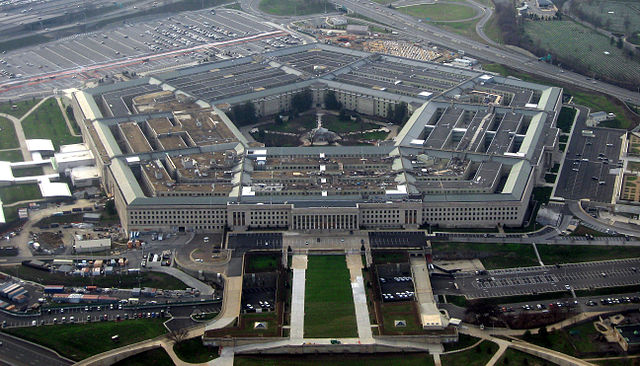
\includegraphics[width=0.35\linewidth]{pentagono.jpg}
\label{fig:pentagono}
\end{figure}

Cierta compa\~nia de contratistas le paga a los alba\~niles \$115.00 por cada
metro cuadrado de pared que consttruyen. Uno de los obreros construye una barda
rectangular cuya base mide $b=6$\,m y altura $h=2.5$\,m. ?`Cu\'al deber\'a ser la
paga que reciba por dicho trabajo?

% section geometr'ia (end)

\newpage
\section{Proporcionalidad} % (fold)
\label{sec:proporcionalidad}

?`Cu\'anto es el 25\% de 350?

\vspace{4cm}
El profesor de matem\'aticas viajna en su autom\'ovil recorriendo en promedio
una distancia de 120\,Km cada hora. ?`Cu\'anto tiempo le tomar\'a llegar a la
ciudad de Guanajuato si la distancia es de 64\,Km?

% section proporcionalidad (end)

\end{document}






